\section{Results}

\subsection{Historical Operation of \gls{EU} Reactors}

\Cref{tab:sim_result} lists the important metrics
obtained from the first simulation. The following
values are the \gls{EU} inventory and history at year 2050,
and will be reprocessed in the second simulation.

\begin{table}[h]
	\centering
%	\scalebox{0.86}{
		\begin{tabular}{|c|c|c|c|}
			\hline
			Category & Unit & Value & Specifics\\ \hline
			Total UOX Usage & MTHM & 181,471 &  \\ \hline
			Total MOX Usage & MTHM & 6,302 & \\ \hline
			Total Used UOX Stored & MTHM & 141,659 & \gls{UNF} that is not reprocessed\\ \hline
			Total Used  MOX Stored & MTHM & 3,611 & \gls{UNF} that is not reprocessed \\ \hline
			Total Tailings & MTHM & 1,081,826 & \\ \hline
			Total Natural U Used & MTHM & 1,269,897 & \\ \hline
		\end{tabular}
		\caption{Simulation Results for Historical Nuclear Operation of \gls{EU} Nations}
		\label{tab:sim_result}
\end {table}
\FloatBarrier


Figures \ref{fig:eu_tail} and \ref{fig:eu_snf} show the 
timeseries of mass of tailings and used fuel accumulation in \gls{EU}.
Figure \ref{fig:eu_fuel} shows the amount of fuel used in \gls{EU}.


\begin{figure}[htbp!]
	\begin{center}
		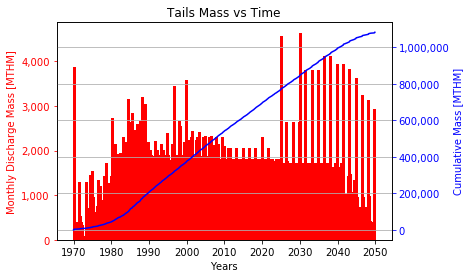
\includegraphics[scale=0.7]{./images/eu_future/tails.png}
	\end{center}
	\caption{Timeseries of Tails Mass in the \gls{EU}.}
	\label{fig:eu_tail}
\end{figure}

\begin{figure}[htbp!]
	\begin{center}
		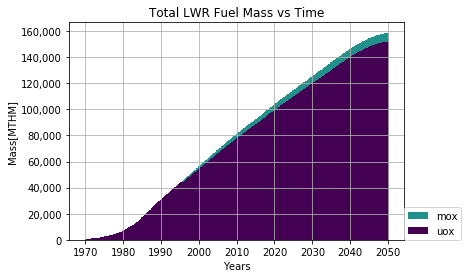
\includegraphics[scale=0.7]{./images/eu_future/total_fuel.png}
	\end{center}
	\caption{Timeseries of Total Fuel Usage in \gls{EU}.}
	\label{fig:eu_fuel}
\end{figure}


\begin{figure}[htbp!]
	\begin{center}
			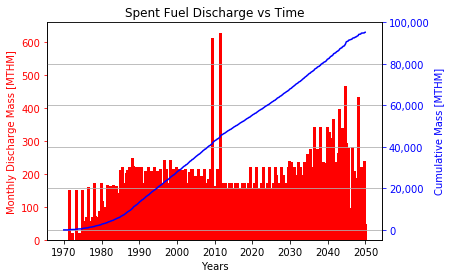
\includegraphics[scale=0.7]{./images/eu_future/snf_discharge.png}
	\end{center}
	\caption{Timeseries of Used Nuclear Fuel in \gls{EU}.}
	\label{fig:eu_snf}
\end{figure}
\FloatBarrier


\begin{table}[h]
	\centering
	\begin{tabular}{|c|c|c|}
		\hline
		Isotope & Mass Fraction in Used Fuel [\%] & Quantity [t] \\ \hline
		Total & 0.9358 & 1,325 \\ \hline
		Pu238 & 0.0111 & 15.72 \\ \hline
		Pu239 & 0.518 & 733.79 \\ \hline
		Pu240 & 0.232 & 328.64 \\ \hline
		Pu241 & 0.126 & 178.49 \\ \hline
		Pu242 & 0.0487 & 68.98 \\ \hline
	\end{tabular}
	\caption{Plutonium From Used Fuel}
	\label{tab:pu}
\end{table}


\Cref{tab:pu} lists the isotope, mass fraction,
and quantity of plutonium that can be obtained from the 2050 \gls{UNF} inventory.


\subsection{French \gls{SFR} Transition Scenario}

Reprocessing \gls{UNF} collected from all EU nations can start approximately
270 \glspl{SFR}, which is more than enough for two generations of 66GWe \gls{SFR}
fleet. With the \gls{SFR} breeding ratio of over one, France can transition into
a fully \gls{SFR} fleet without extra construction of \glspl{LWR}. 

From Varaine et al. \cite{marsaultmarie-sophie_pre-conceptual_2012}, a French
ASTRID-type \gls{SFR} of capacity 600 MWe needs $1.225$ tons of
plutonium a year, with an initial plutonium loading of $4.9$ tons. 
Thus, the number of \glspl{SFR} that can be loaded with the reprocessed
plutonium from \gls{UNF} can be estimated to $\frac{Pu \ from \ legacy \ \gls{UNF}}{4.9} \approx 270$ \glspl{SFR},
assuming infinite reprocessing and fabrication capacity as well as
abundant depleted uranium supply. 

Also, assuming that \gls{MOX} can be recycled indefinitely,
used \gls{MOX} from an ASTRID reactor contains enough plutonium to produce a \gls{MOX} fuel with
the same mass, if mixed with depleted uranium. For example,
used \gls{MOX} from an ASTRID reactor is assumed to be 12.6\% plutonium
in this simulation (see \cref{tab:comp}), whereas a fresh \gls{MOX} is 11\% plutonium.
Separating plutonium from used \gls{MOX} from
an ASTRID reactor can create \gls{MOX} of the mass of used \gls{MOX}.
The plutonium breeding ratio in this simulation is thus assumed to be
$\approx 1.145$.

\Cref{fig:fuel} shows \gls{MOX} loaded in the \glspl{SFR} per month.
The spikes are due to initial fuel demand for new deployment of \glspl{SFR}.
The initial loading of new \glspl{SFR} are done with the \gls{MOX} created
from legacy \gls{UNF}. Once there are enough amounts of extra plutonium creation
by deployed \glspl{SFR}, the legacy \gls{UNF} is no longer used. 

\begin{figure}[htbp!]
	\begin{center}
		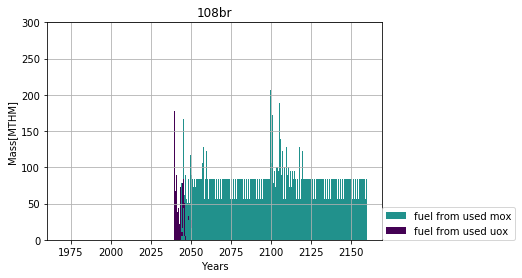
\includegraphics[scale=0.7]{./images/french-transition/where_fuel.png}
	\end{center}
	\caption{Timeseries of fuel loaded into \glspl{SFR}}
	\label{fig:fuel}
\end{figure}

\Cref{fig:reprocess_waste} shows the amount of reprocessing waste
(minor actinides, fission products) over time. The spikes in the 
waste discharge is due to large influx of spent fuel from
decommissioned \glspl{SFR}.\Cref{fig:pu_no_cum} shows the separated plutonium discharge
per month from the reprocessing plant. The plutonium outflux
does not precisely follow the fuel demand because \Cyclus agents have
material buffers that store commodity fuel for later usage. 
\Cref{tab:sfr_sim_result} lists metrics obtained from the second simulation.

\begin{figure}[htbp!]
	\begin{center}
		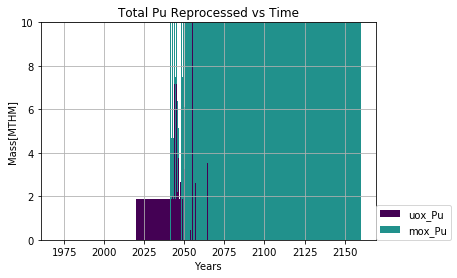
\includegraphics[scale=0.7]{./images/french-transition/pu.png}
	\end{center}
	\caption{Separated plutonium discharge from Reprocessing Plant}
	\label{fig:pu_no_cum}
\end{figure}


\begin{figure}[htbp!]
	\begin{center}
		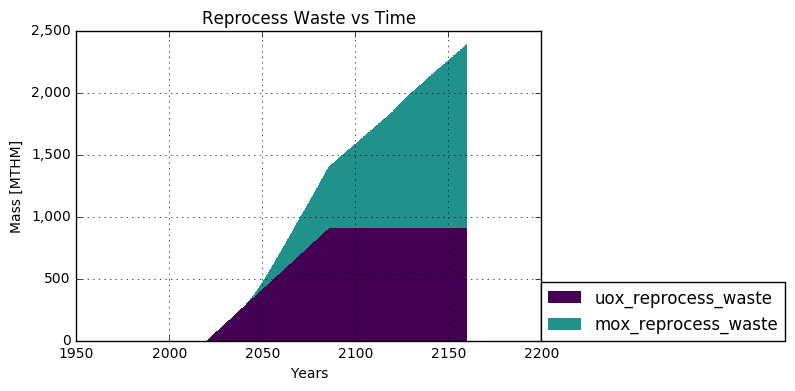
\includegraphics[scale=0.7]{./images/french-transition/reprocess_waste.png}
	\end{center}
	\caption{Reprocessing waste discharge from Reprocessing Plant}
	\label{fig:reprocess_waste}
\end{figure}


\begin{table}[h]
	\centering
	\scalebox{0.86}{
		\begin{tabular}{|c|c|c|}
			\hline
			Category & Unit & Value  \\ \hline
			Total MOX used & MTHM & 127,640  \\ \hline
			Total \glspl{SFR} Deployed & & 220 \\ \hline
			Total Plutonium Reprocessed & MTHM & 16,352 \\ \hline
			Total MOX from UOX Waste & MTHM & 6,570  \\ \hline
			Total MOX from MOX Waste & MTHM  & 121,070 \\ \hline
			Total Tails used & MTHM & 116,153 \\ \hline
			Total legacy UNF reprocessed & MTHM & 77,082 \\ \hline
			Total Reprocessed Uranium Stockpile & MTHM & 184,172 \\ \hline
			Total Reprocess Waste & MTHM & 16,352 \\ \hline
		\end{tabular}}
		\caption {\gls{SFR} Simulation Results}
		\label{tab:sfr_sim_result}
\end {table}


